\documentclass[a4paper,12pt]{article} % тип документа

\usepackage{tikz}
\usepackage[T2A]{fontenc}			% кодировка
\usepackage[utf8]{inputenc}			% кодировка исходного текста
\usepackage[english,russian]{babel}	% локализация и переносы
\usepackage{amsfonts,longtable}

% Математика
\usepackage{amsmath,amsfonts,amssymb,amsthm,mathtools} 


\usepackage{wasysym}

\title{Лабораторный журнал к работе 1.2.3 по курсу \\ "Общая физика"  \\ 
\vspace{0.2cm}
\vspace{4.5cm}
 \LARGE{\textbf{Определение моментов инерции твердых тел с помощью трифилярного подвеса}}\vspace{5.5cm}}
\date{23.11.2018}
\usepackage{tikz}
\author{\vspace{0.2cm}Баринов Леонид}

\begin{document}
\maketitle
\newpage
\textbf{Цель работы:} измерение момента инерции ряда тел и сравнение результатов с расчетами по теоретическим формулам; проверка аддитивности моментов инерции и справедливости формулы Гюйгенса-Штейнера.\\
\textbf{В работе используются:} трифилярный подвес, секундомер, счетчик числа колебаний, набор тел, момент инерции которых надлежит измерить (диск, стержень, полый цилиндр и другие)

Инерционность при вращении тела относительно оси определяется моментом инерции тела оносительно этой оси. Момент инерции твердого тела относительно неподвижной оси вращения вычисляется по формуле:
\begin{equation}
I = \int r^2dm
\end{equation}
Здесь $r$ -- расстояние элемента массы тела $dm$ от оси вращения. Интегрирование проводится по всей массе тела $m$.
\begin{figure}[h]
\centering
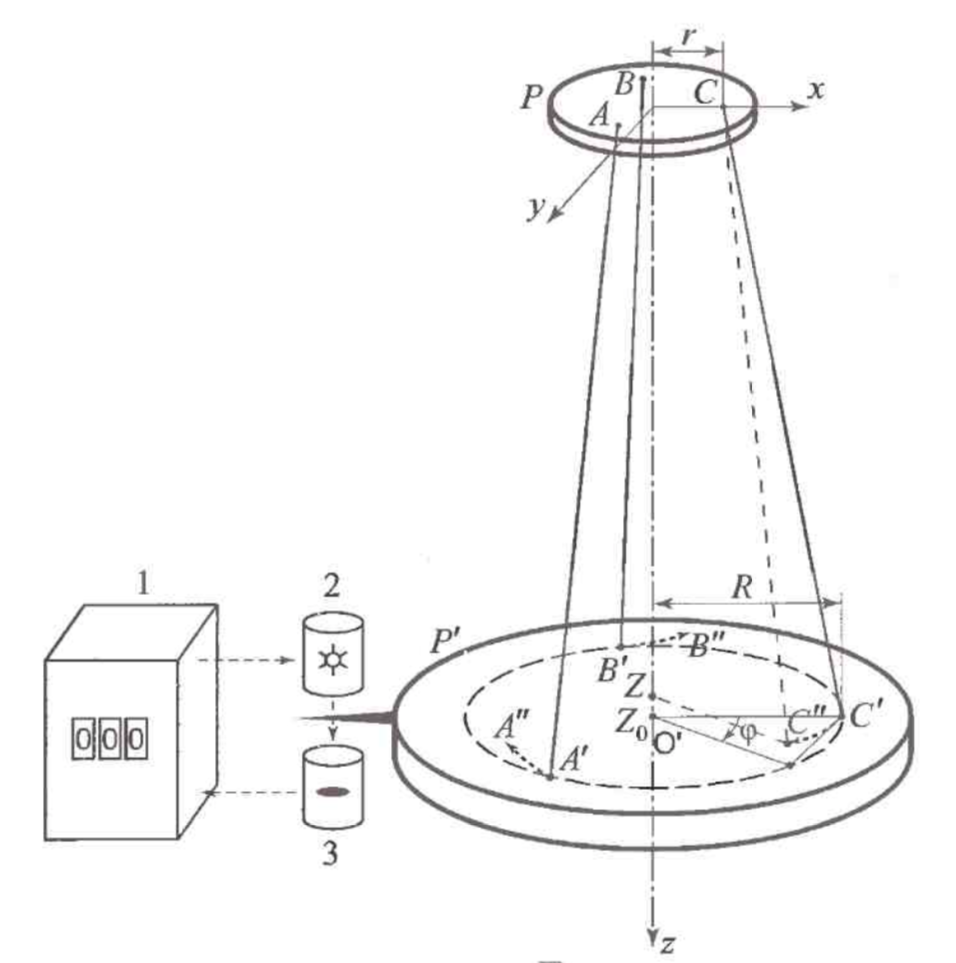
\includegraphics[scale=0.5]{1}
\caption{Трифилярный подвес}
\end{figure}

Для ондородных тел известной плотности при заданных размерах и достаточно простой форме момент инерции можно вычислить. Для неоднородных тел и тел сложной формы момент инерции можно опрделеить экспериментально. Удобно использовать устройство, показанное на Рис. 1 и называемое трифилярным подвесом. Оно состоит из укрепленной на некоторой высоте неподвижной платформы $P$, и подвешенной к ней на трех симметрично расположенных нитях $AA', BB'$ и $CC'$ вращающейся платформы $P'$.

Платформа $P$ укреплена на кронштейне и снабжена рычагом (на рисунке не показан), при помощи которого в системе можно создать крутильные колебания путем небольшого поворота верхней платформы. Лучше поворачивать верхнюю платформу, укрепленную на неподвижной оси, чем подвешенную на нитях нижнюю, так как нижнюю платформу трудно закрутить не вызвав ее раскачиваний, подобных движению маятника, учет которых сильно усложнил бы расчеты. После поворота, вызывающего крутильные колебания, верхняя платформа остается неподвижной в течение всего процесса колебаний. После того, как нижняя платформа $P'$ оказывается повернутой на угол $\varphi$ относительно верхней платформы $P$, возникает момент сил, стремящийся вернуть нижнюю платформу в положение равновесия, при котором оносительный поворот отсутствует. Но в положении равновесия платформа не останавливается, так как имеет угловую скорость (кинетическую энергию вращения). В результате платформа совершает крутильные колебания.

Если пренебречь потерями энергии на трение (о воздух и в креплениях нитей), то ураввнение сохранения энергии при колебаний можно записать слеюущим образом:
\begin{equation}
\frac{I\dot{\varphi^2}}{2} + mg(z_0-z) = E
\end{equation} 

Здесь $I$ -- момент инерции платформы вместе с исследуемым телом, $m$ -- масса платформы с телом, $\varphi$ -- угол поворота платформы от положения равовесия системы, точкой обозначена производная по времени (угловая скорость), $z_0$ -- координата по вертикали центра нижней платформы $O'$ при равновесии ($\varphi$ = 0), $z$ -- координата той же точки при некотором угле поворота $\varphi$. Первый член в левой части уравнения -- кинетическая энергия вращения, второй член -- потенциальная энергия в поле тяженсти, $E$ -- полная энергия системы (платформы с телом).

Отметим, что, как показывает соотношение (2), возвращающая сила возникает благодаря силе тяжести.

Воспользуемся системой координат $x, y, z$, связанной с верхней платформой, как показано на рис. 1. Координта верхнего конца одной из нитей подвеса точки $C$ в этой системе -- $(r, 0, 0)$. Нижний конец данной нити $C'$, находящийся на нижней платформе, приравновесии имеет координаты $(R, 0, z_0)$, а при повороте платформы на угол $\varphi$ эта точка переходит в $C''$ с координатами $(R\cos\varphi, R\sin\varphi, z)$. Расстояние между точками $C$ и $C''$ равно длине нити $L$. Поэтому:
\begin{equation}
(R\cos\varphi-r)^2 + R^2\sin^2\varphi + z^2 = L^2
\end{equation}
Учитвая, что при малых углах поворота $\cos\varphi\approx 1 - \frac{\varphi}{2}$, получаем 
\begin{equation}
z^2 = L^2 - R^2 - r^2 + 2Rr\cos\varphi = x_0^2 - 2Rr(1-\cos\varphi) \approx z_0^2 - Rr\varphi^2
\end{equation}
Извлекая из (4) квадратный корень и учитывая малость угла $\varphi$, имеем
\begin{equation}
z \approx \sqrt{z_0^2 - Rr\varphi^2}\approx z_0\sqrt{1 - \frac{Rr\varphi^2}{z_0^2}}\approx z_0 - \frac{Rr\varphi^2}{2z_0}
\end{equation}
Подставляя это значение $z$ в уравнение (2), получаем
\begin{equation}
\frac{1}{2}I\dot\varphi^2 + mg\frac{Rr}{2z_0}\varphi^2 = E
\end{equation}

Диффурунцируя по времени и сокращая на $\dot{\varphi}$, находим уравнение крутильных колебаний системы:
\begin{equation}
I\ddot{\varphi}+mg\frac{Rr}{z_0}\varphi = 0
\end{equation}
Производная по времени от $E$ равно нулю, так как потерями энергии на трение, как уже было сказано выше, пренебрегаем.

Решение этого уравнения, как нетрудно убедиться простой подстановкой, имеет вид
\begin{equation}
\varphi = \varphi_0\sin\left(\sqrt{\frac{mgRr}{Iz_0}}t+\theta\right)
\end{equation}
Здесь амплитуда $\varphi_0$ и фаза $\theta$ колебаний определяются начальными условиями. Период крутильных колебаний нашей системы равен
\begin{equation}
T = 2\pi\sqrt{\frac{Iz_0}{mgRr}}
\end{equation}
Обратим внимание на то, что из этой формулы при $r = R$ и $I = mR^2$ (тонкое кольцо) получаем формулу для математчиеского маятника.

Из (9) находим формулу для определения момента инерции:
\begin{equation}
I = \frac{mgRrT^2}{4\pi^2z_0}
\end{equation}

Учитывая, что параметры установки $R$, $r$ и $z_0$ при проведении опытов не меняются, удобно переписать последнее уравнение следующим образом:
\begin{equation}
I = kmT^2
\end{equation}
Здесь $k = \frac{gRr}{4\pi^2z_0}$ -- велечина, постоянная для данной установки.

Таким образом, полученные формулы позволяют определить момент инерции платформы с телом и отдельно платформы по соответсвующим периодам крутильных колебаний. Затем вычисляем момент инерции тела, пользуясь аддитивностью, в справедливости которой можно убедиться, проведя измерения сначала для каждого из двух тел отдельно, а затем для обоих тел вместе.

При выводе формул предполагалось, что малы необратимые потери энергии, связанные с трением, то есть мало затухание колебаний. О затухании колебаний можно судить, сравнивая время $\tau$ уменшения амплитуды колебаний в 2-3 раза с периодом колебаний $T$. Необратиыми потерями энергии можно пренебречь, если выполняется условие 
\begin{equation}
\tau \gg T
\end{equation}

В данной работе рекомендуется период колебаний определять с относительной погрешность $0,5\%$. Число колебаний, по которым надо вычислять период, определяется этой погрешностью и погрешностью измерения времени.

Для счета числа колебаний используется счетчик, состоящий из осветителя (2), фотоэлемента (3) и пересчетеного устройства (1) (см Рис. 1). Легкий лепессток, укрепленный на платформе, при колебаниях пересекает световой луч дважды за период. Соответсвующие сигналы от фотоэлемнта поступают на пересчетное устройство.\\
\textbf{Ход работы:}
\begin{itemize}
\item[1.] Не нагружая нижней платформы, проверяем, пригодна ли установка для измерений, то есть нормально ли функционирует устройство для возбуждения крутильных колебаний, не возкникают ли при этом нежелательные маятниковообразные движения платформы, работает ли счетчик числа колебаний.
\item[2.] Возбудив в установке крутильные колебания, проверяем, достаточно ли хорошо выполняется соотношения (12). При этом добиваться большой точности в измерении периода и времени уменьшения амплитуды в 2-3 раза не имеет смысла. Проводить измерения рекомендуется для ненагруженной платформы. 
\item[3.]Найдем рабочий диапозон амплитуд колебаний. Амплитуду надо уменьшать до тех пор, пока период колебаний, определенный по 20-30 полным колебаниям, не перестанет зависеть от амплитуды. Рабочий диапазон начинается с тех амплитуд, для которых период совпадает с периодом колебаний с амплтудой вдвое меньшей.
\item[4.]Измеряем параметры установки: $z_0, R$ и $r$ (см. Рис. 1). По ним вычисляем константу установки $k$, входящую в формулу (11), и ее погрешность $\sigma_k$.
\item[5.] Определяем момент инерции ненагруженной платформы (здесь и далее периоды колебаний следует определять с относительной погрешностью не хуже $0,5\%$).
\item[6.]Измеряем моменты инерции двух тел из имеющегося набора сначала порознь, а затем вместе. Помещать тела на платформу надо так, чтобы общий центр масс всегода находился на оси вращения (оси симметрии) системы, то есть чтобы не было заметного перекоса платформы. Для удобства на платформе нанесен ряд концентрических окружностей. Проверяем аддитивность моментов инерции, то есть справедливость соотношения $I = I_1+I_2$, где $I_1$ и $I_2$ -- моменты инерции первого и второго тел, а $I$ -- общий момент инерции. Погрешность, с которой выполняется это соотношение, является хорошей мерой точности проводимых измерений. Рассчитаем теоретически моменты инерции $I$ всех используемых в эксперименте тел и сравниваем результаты с измеренными значениями $I$.
\item[7.] Поместим на платформу диск, разрезанный до диаметру. Постепенно раздвигая половинки диска так, чтобы их общий центр масс все время оставался на оси вращения платформы (Рис. 2), снимаем зависимость момента инерции такой системы $I$ от расстояния $h$ каждой из половинок до оси вращения (центра платформы)
\begin{figure}[h]
\centering
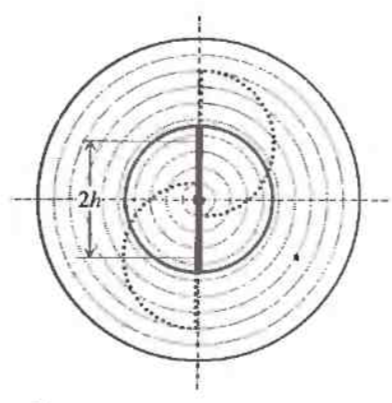
\includegraphics[scale=0.5]{2}
\caption{Расположение тел на платформе}
\end{figure}
\end{itemize}






\end{document}
